\documentclass[crop=false]{standalone}

\begin{document}
\subsection{LANs,WANs and the Internet}
\subsubsection{Network Components}
The network infrastructure contains three categories of network components:
\begin{itemize}
  \item \textbf{Devices}
  \begin{itemize}
    \item \textbf{End devices}\\either the source or destination of a message transmitted over the network, identified by an address, such as laptop, PC, file/web/email server or client, etc.
    \item \textbf{Intermediary network devices}\\connect the individual end devices to the network and connect multiple individual networks to form an inter-network, such as router or wireless router, LAN switch, multilayer switch, firewall appliance, etc.
  \end{itemize}
  
  \begin{figure}[ht]
    \centering
    \begin{subfigure}{.5\textwidth}
      \centering
      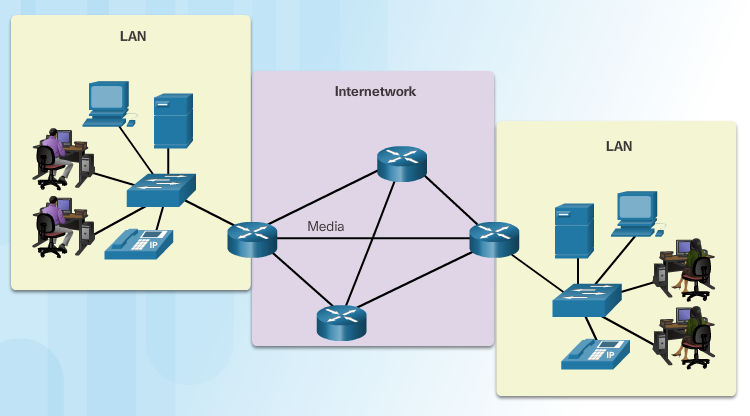
\includegraphics[height=4cm, width=\linewidth]{endDevice}
      \caption{End devices}
      \label{fig:end devices}
      \end{subfigure}%
    \begin{subfigure}{.5\textwidth}
      \centering
      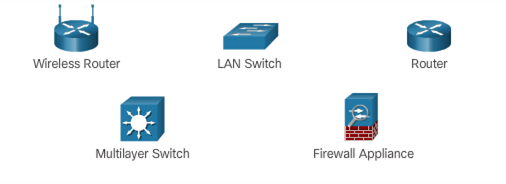
\includegraphics[height=4cm, width=\linewidth]{intermediaryDevice}
      \caption{Intermediary devices}
      \label{fig:intermediary devices}
    \end{subfigure}
    \caption{Devices}
    \label{fig:Devices}
  \end{figure}

  \item \textbf{Media}
  \begin{itemize}
    \item \textbf{Metallic wires within cables} \hspace{5mm}data is encoded into electrical impulses
    \item \textbf{Fiber optic cable} \hspace{5mm}data is encoded as pulses of light
    \item \textbf{Wireless transmission} \hspace{5mm}data is encoded using wavelengths from the electromagnetic spectrum
  \end{itemize}
  
  \begin{figure}[h]
    \centering
    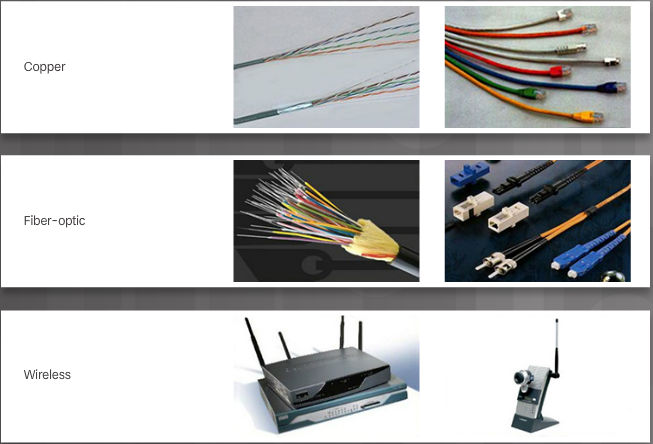
\includegraphics[height=5cm, width=0.5\textwidth]{media}
    \caption{Media}
    \label{fig:Media}
  \end{figure}

  \item \textbf{Services} \\include many of the common network applications people use every day.
\end{itemize}

\subsubsection{Network Representations}
A \textbf{topology diagram} is used to visualize the organization and operation of a network.

\begin{wrapfigure}{r}{2.5cm}
  \centering
  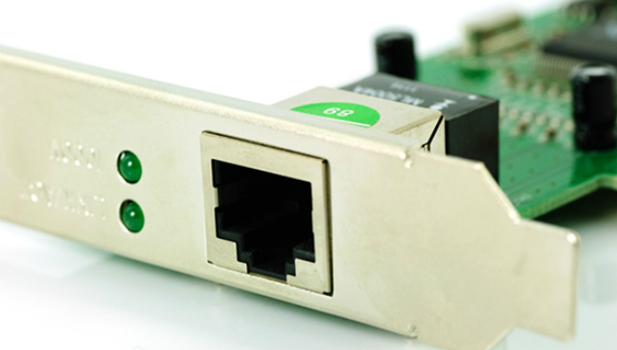
\includegraphics[width=\linewidth]{NIC}
  \caption{NIC}
  \label{fig:Network Interface Card(NIC)}
\end{wrapfigure}

Specialized terminology is used when discussing how each of these devices and media connect to each other.

\begin{itemize}
  \item \textbf{\acrfull{nic}} \\provides the physical connection to the network at an end device. 
  \item \textbf{\Gls{physical port}} \\a connector or outlet on a networking device where the media is connected to an end device or another networking device.
  \item \textbf{\Gls{interface}} \\specialized port on a networking device that connect to individual networks.
\end{itemize}

\textbf{Note}: Often, the terms "port" and "interface" are used interchangeably. The port on a router are referred to as "\gls{network interface}".

There are two types of topology diagrams:
\begin{itemize}
  \item \textbf{\gls{physical topology diagram}} \\identify the physical location of intermediary devices and cable installation.
  \item \textbf{\gls{logical topology diagram}} \\identify devices, ports, and addressing scheme.
\end{itemize}

\begin{figure}[ht]
  \centering
  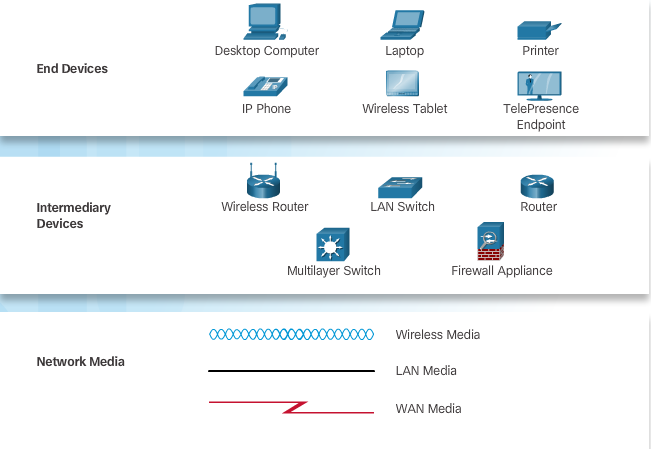
\includegraphics[height=6.5cm, width=0.75\textwidth]{networkRepSymbol}
  \caption{Network Representation symbols}
  \label{fig:Network Representation symbols}
\end{figure}

\begin{figure}[ht]
    \centering
    \begin{subfigure}{.5\textwidth}
      \centering
      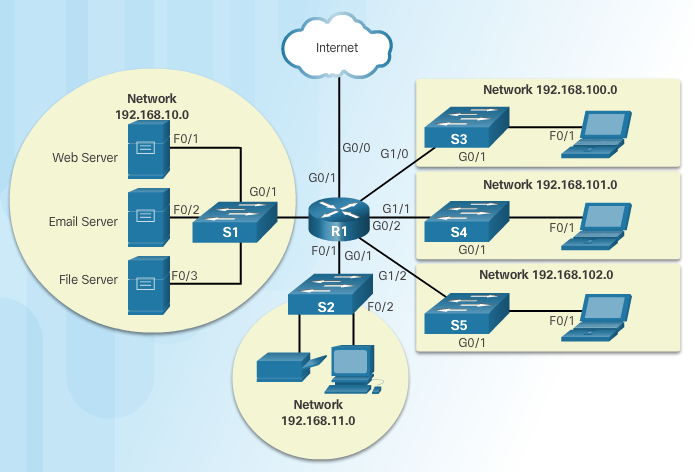
\includegraphics[height=6.5cm, width=\linewidth]{logicalTopology}
      \caption{Logical topology diagram}
      \label{fig:Logical topology diagram}
      \end{subfigure}%
    \begin{subfigure}{.5\textwidth}
      \centering
      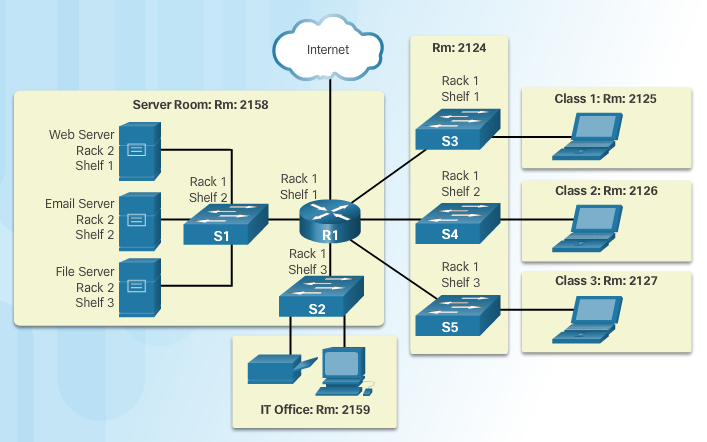
\includegraphics[height=6.5cm, width=\linewidth]{PhysicalTopology}
      \caption{Physical topology diagram}
      \label{fig:Physical topology diagram}
    \end{subfigure}
    \caption{Topology Diagram}
    \label{fig:Topology Diagram}
\end{figure}

\subsubsection{LANs and WANs}
Typical network infrastructures include:

\begin{itemize}
  \item \textbf{\acrfull{lan}} \hspace{5mm}typically an enterprise, home, or small business network owned and managed by an individual or IT department.
  \item \textbf{\acrfull{wan}} \hspace{5mm}provides access to other networks over a wide geographical area, owned and managed by a telecommunication service provider, including \acrfull{isp}.
  \item \textbf{\acrfull{man}} \hspace{5mm}larger than a LAN but smaller than a WAN (e.g., a city).
  \item \textbf{\acrfull{wlan}} \hspace{5mm}LAN wirelessly interconnecting end points.
  \item \textbf{\acrfull{san}} \hspace{5mm}support file servers and provide data storage, retrieval and replication.
\end{itemize}

LANs provide high speed bandwidth to internal end devices and intermediary devices while WANs typically provide slower speed links between LANs.

\begin{figure}[ht]
  \centering
  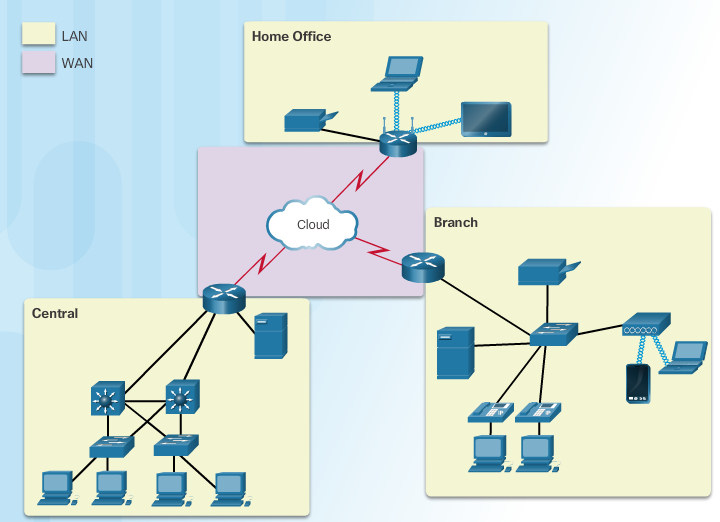
\includegraphics[height=7cm, width=0.75\textwidth]{lansAndWans}
  \caption{LANs and WANs}
  \label{fig:LANs and WANs}
\end{figure}

\subsubsection{The Internet, Intranets, and Extranets}
The \textbf{Internet} is a worldwide collection of interconnected networks. There are organizations helping to maintain structure and standardization of Internet protocols and processes, including the Internet Engineering Task Force (IETF), Internet Corporation for Assigned Names and Numbers (ICANN), the Internet Architecture Board (IAB), etc.\\
\textit{Note}: The term "\textbf{internet}" describes multiple networks interconnected.\\
\textbf{Intranet} refers to a private connection of LANs and WANs that belongs to an organization, and is accessible only by the organization's members, employees, or others with authorization.\\
However, organization may use an "\textbf{extranet}" to provide secure and safe access to individuals who work for a different organization, but require access to the organization’s data.

\begin{figure}[ht]
\centering
\begin{minipage}{.5\textwidth}
  \centering
  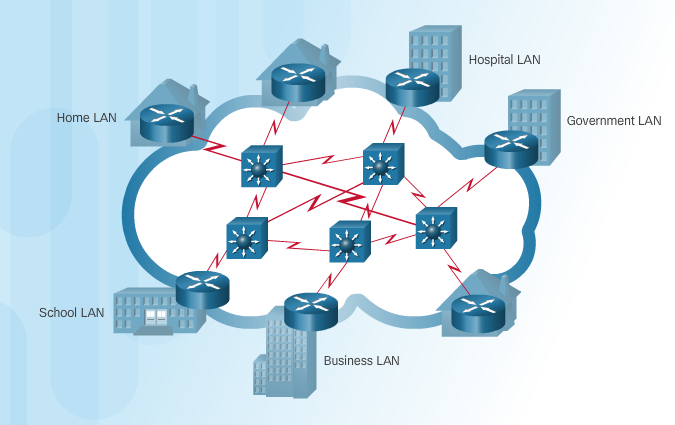
\includegraphics[height=7cm, width=\linewidth]{Internet}
  \captionof{figure}{Internet: collection of interconnected networks}
  \label{fig:Internet: collection of interconnected networks}
\end{minipage}%
\begin{minipage}{.5\textwidth}
  \centering
  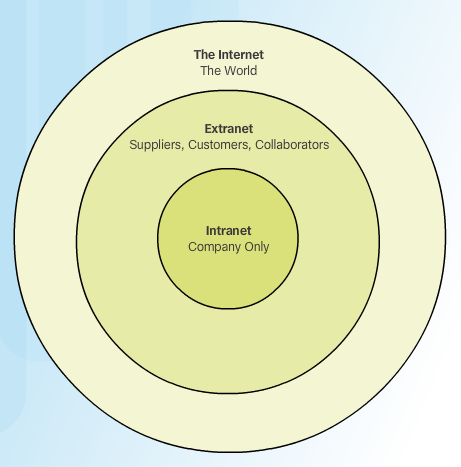
\includegraphics[height=7cm, width=\linewidth]{InternetIntranetExtranet}
  \captionof{figure}{Internet Intranet and Extranet}
  \label{fig:Internet Intranet and Extranet}
\end{minipage}
\end{figure}

\subsubsection{Internet Connections}
There are many different ways to connect users and organizations to the Internet.
\begin{itemize}
  \item Home and Small Office Internet Connections
    \begin{itemize}
      \item \textbf{Cable} \hspace{5mm}typically offered by cable television service providers or connected directly with fiber optic cables, providing a high bandwidth.
      \item \textbf{\acrfull{dsl}} \hspace{5mm}runs over a telephone line. Popular choice is \acrfull{adsl}, where the download speed is faster than the upload speed.
      \item \textbf{Cellular} \hspace{5mm}uses a cell phone network to connect.
      \item \textbf{Satellite} \hspace{5mm}requires a clear line of sight to the satellite.
      \item \textbf{Dial-up Telephone} \hspace{5mm}an inexpensive option using any phone line and a modem, with a low bandwidth. 
    \end{itemize}
  \item Businesses Internet Connections
    \begin{itemize}
      \item \textbf{Dedicated Leased Line} \hspace{5mm}reserved circuits within the service provider's network, geographically separated offices for private voice/data networking, expensive rented at a monthly or yearly rate.
      \item \textbf{Ethernet WAN} \hspace{5mm}expend Ethernet technology into the WAN.
      \item \textbf{DSL} \hspace{5mm}popular choice is \acrfull{sdsl}, with equal upload and download speeds.
      \item \textbf{Satellite} \hspace{5mm}when a wired solution is not available.
    \end{itemize}
\end{itemize}

\begin{figure}[ht]
    \centering
    \begin{subfigure}{.5\textwidth}
      \centering
      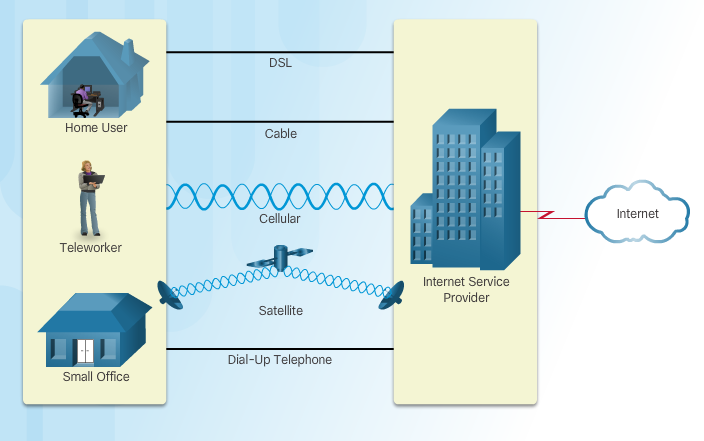
\includegraphics[height=5cm, width=\linewidth]{userConnect}
      \caption{Home and Small Office}
      \label{fig:Home and Small Office Internet Connections}
      \end{subfigure}%
    \begin{subfigure}{.5\textwidth}
      \centering
      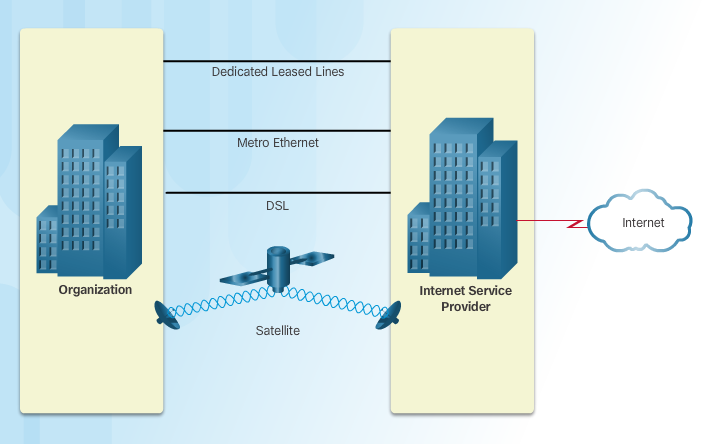
\includegraphics[height=5cm, width=\linewidth]{businessConnect}
      \caption{Businesses}
      \label{fig:Businesses Internet Connections}
    \end{subfigure}
    \caption{Internet Connection Technology}
    \label{fig:Internet Connection Technology}
\end{figure}

\subsection{Network Environments}
Today, separate networks are converging. Converged networks delivers data, voice, and video between different types of devices over the same network infrastructure, using the same set of rules, agreements, and implementation standards.
\subsubsection{Reliable Network}
There are four basic characteristics that the network architecture\footnote{technologies that support the infrastructure and the programmed services, rules or protocols.} needs to address in order to meet user expectations:
\begin{itemize}
  \item \textbf{Fault tolerant}\\\textit{keyword}: redundancy, packet-switched network
  \item \textbf{Scalability}\\\textit{keyword}: standards, protocols
  \item \textbf{\acrfull{qos}}\\\textit{keyword}: congestion, network bandwidth, priority queue policy
  \item \textbf{Security}
    \begin{itemize}
      \item network infrastructure security\footnote{the physical securing of devices, and preventing unauthorized access to the management software that resides on them.}
      \item information security\footnote{protecting the information within the packets and the information stored on network attached devices.}
    \end{itemize}
    \textit{keyword}: confidentiality, integrity, availability
\end{itemize}

\begin{flushleft}
Fault tolerant limits the impact of a failure and allows quick recovery when such a failure occurs. The solution is \textbf{\gls{redundancy}} by implementing a \textbf{\gls{packet-switched network}}. Redundant connections allow for alternative paths if a device or a link fails. A single message, is broken into multiple message blocks, called packets. Each packet has the necessary addressing information of the source and destination of the message. The routers within the network switch the packets. All the packets in a single message could take very different paths to the destination. This is quite different from circuit-switched network traditionally used for voice communications where a dedicated circuit is established between the source and destination before the users may communicate.
\end{flushleft}
\begin{figure}[ht]
  \centering
  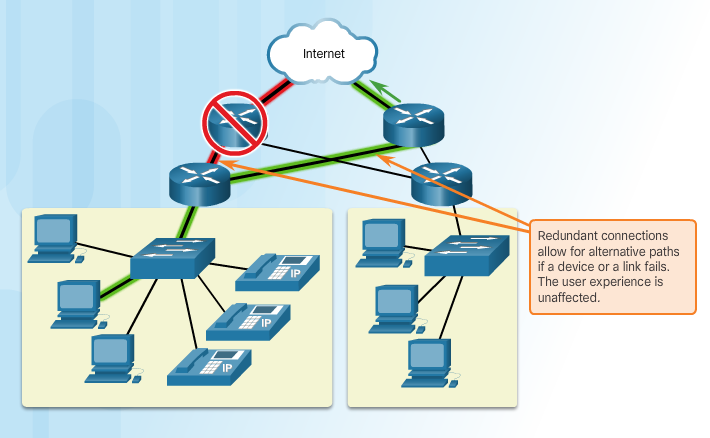
\includegraphics[height=7cm, width=0.75\textwidth]{faultTolerence}
  \caption{Reliable Network: Fault tolerant}
  \label{fig:Reliable Network: Fault tolerant}
\end{figure}

\begin{flushleft}
A scalable network can \textbf{expand quickly} to support new users and applications without impacting the performance of the service being delivered to existing users, because the designers follow accepted \textbf{standards and protocols}.
\end{flushleft}
\begin{figure}[ht]
  \centering
  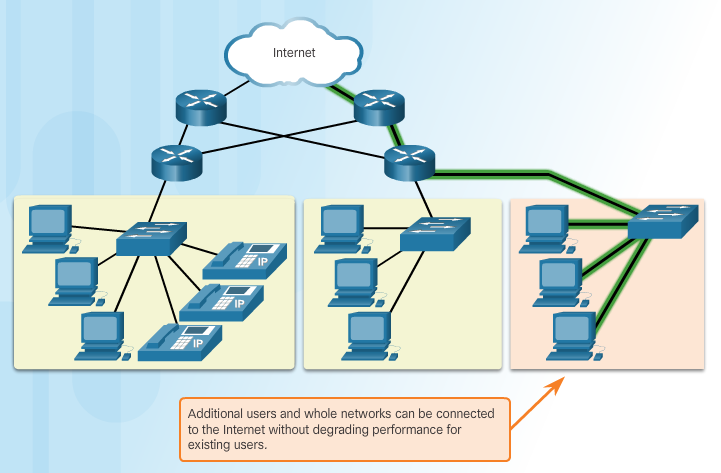
\includegraphics[height=7cm, width=0.75\textwidth]{scability}
  \caption{Reliable Network: Scalability}
  \label{fig:Reliable Network: Scalability}
\end{figure}

\begin{flushleft}
\acrshort{qos} is a primary mechanism for managing congestion and ensuring reliable delivery of content to all users. \textbf{\Gls{congestion}} occurs when the demand for bandwidth exceeds the amount available. \textbf{\Gls{network bandwidth}} is measured in \textit{bits per second}(bps), the number of bits that can be transmitted in a single second. \textbf{Priority queue policy} is implemented by routers if the network experiences congestion.
\end{flushleft}
\begin{figure}[ht]
  \centering
  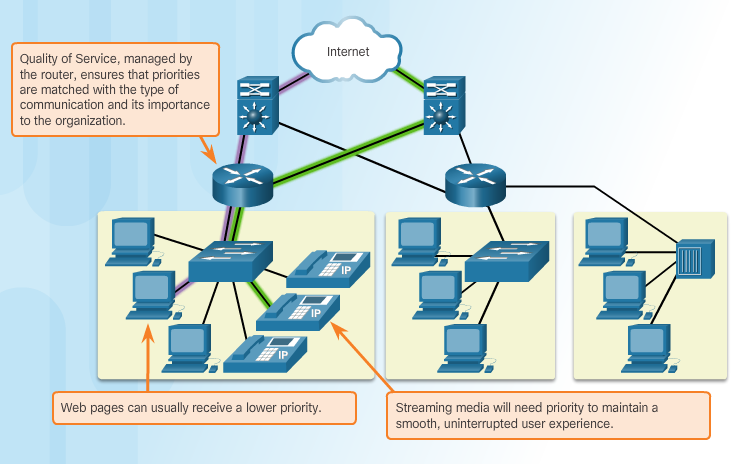
\includegraphics[height=7cm, width=0.75\textwidth]{qos}
  \caption{Reliable Network: \acrfull{qos}}
  \label{fig:Reliable Network: QoS(Quality of Service)}
\end{figure}

\begin{flushleft}
As for network security, there are three primary requirements. Firstly, \textbf{\gls{confidentiality}}, only the intended and authorized recipients can access and read data. Secondly, \textbf{\gls{integrity}}, the information has not been altered in transmission. Thirdly, \textbf{\gls{availability}}, timely and reliable access to data services for authorized users.
\end{flushleft}
\begin{figure}[ht]
  \centering
  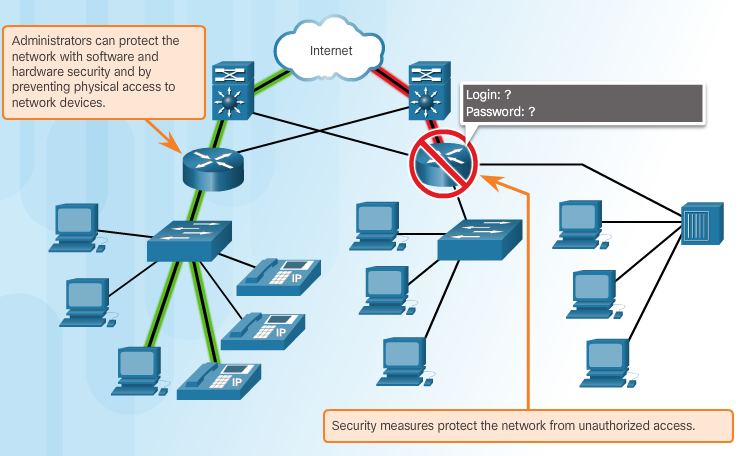
\includegraphics[height=7cm, width=0.75\textwidth]{security}
  \caption{Reliable Network: Security}
  \label{fig:Reliable Network: Security}
\end{figure}

\subsubsection{Network Trends}
fdasf
\end{document}